Grundlegend für Streuexperimente ist der Wirkungsquerschnitt $\sigma$.
Der Wirkungsquerschnitt beschreibt die Wechselwirkungswahrscheinlichkeit einer Projektils mit einem bestimmten Target.
Dabei hat $\sigma$ die Dimension einer Fläche und beschreibt anschaulich eine 'Wechselwirkungsfläche' des jeweiligen Atoms im Target.
Je größer die Fläche, desto wahrscheinlicher die Streuung.
\begin{figure}[h!]
  \centering
  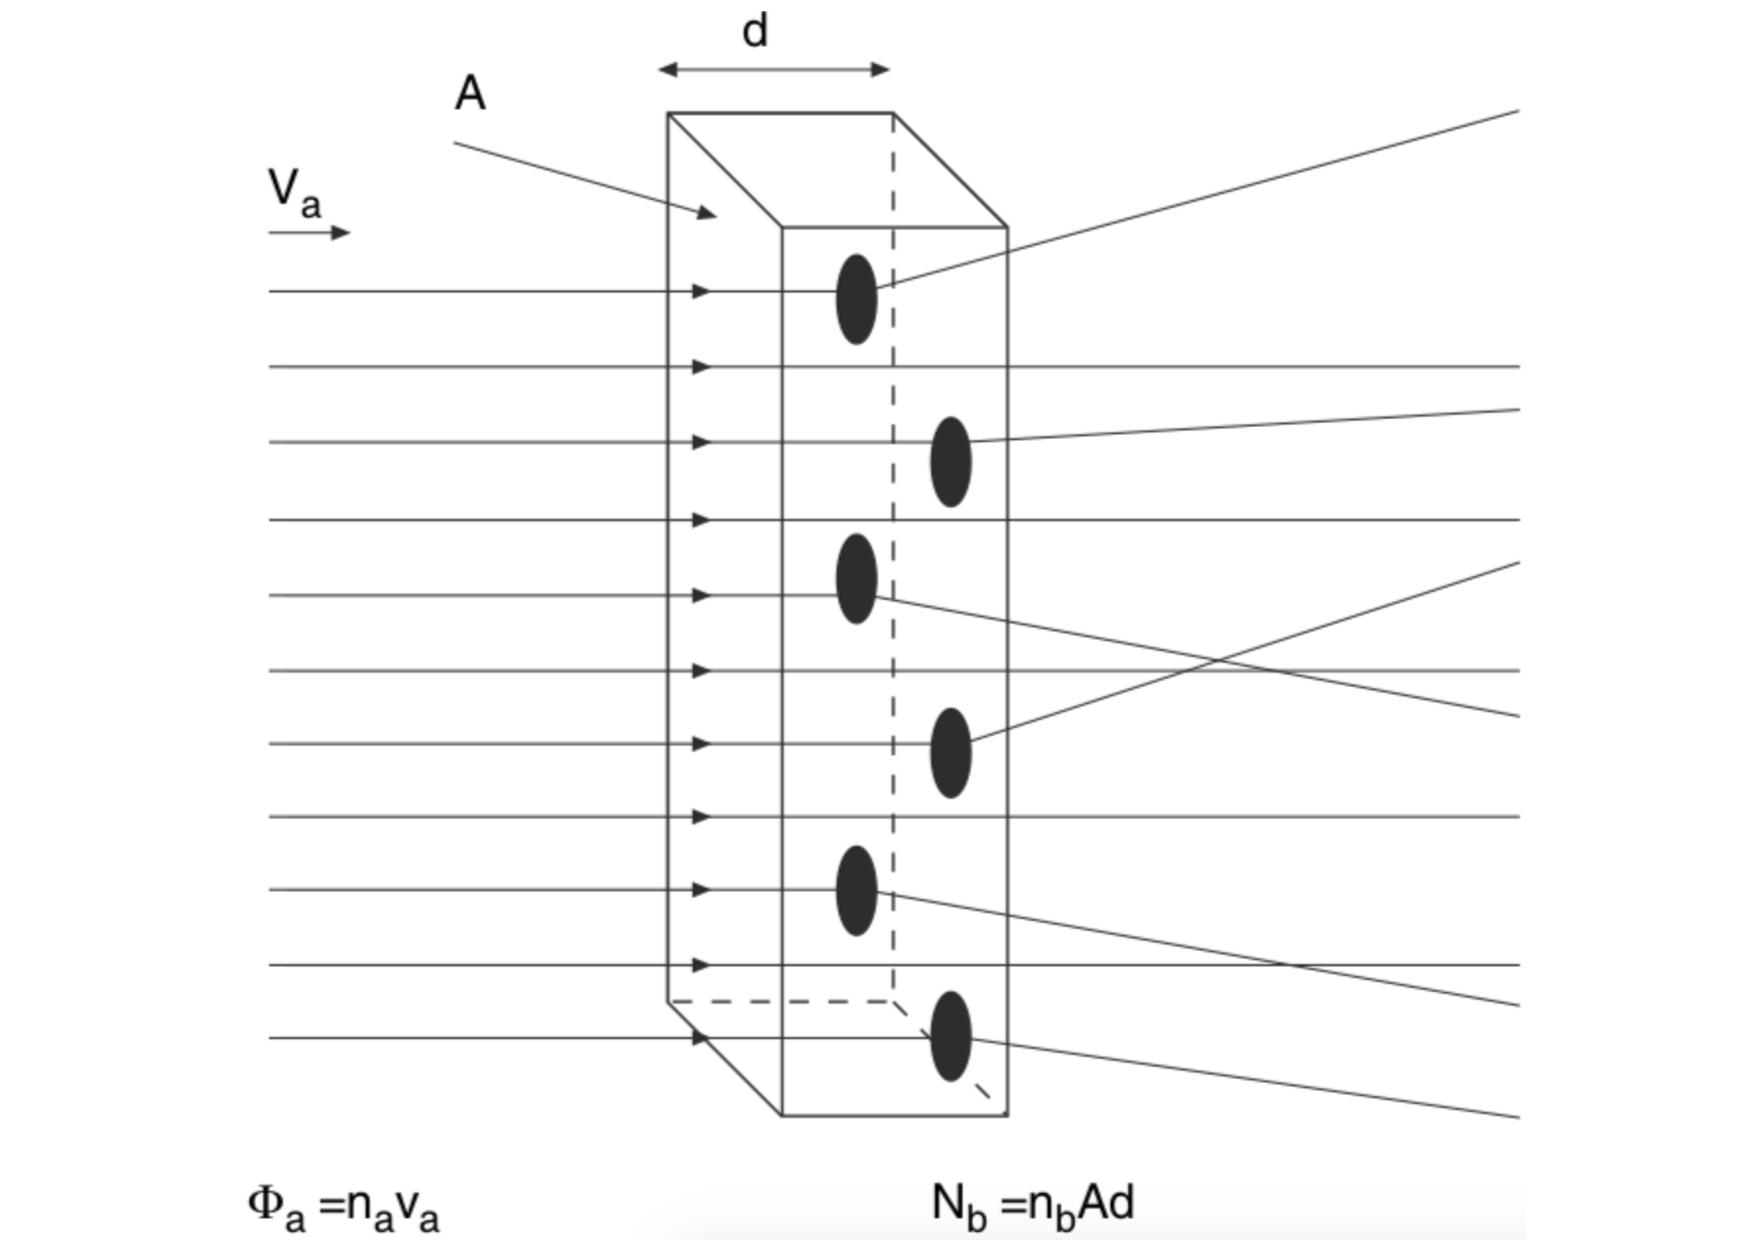
\includegraphics[width=0.6\textwidth]{images/wq.pdf}
  \caption{Anschauliche Beschreibung des Wirkungsquerschnitts $\sigma$ \cite{povh}}
  \label{fig:wq}
\end{figure}

Die $\alpha$-Teilchen, die bei der Rutherford-Streuung verwendet werden, verlieren in der Folie ihre kinetische Energie.
Allgemein kann der Energieverlust von geladenen Teilchenstrahlen in Materie über verschiedene Prozesse entstehen.
Bei Wechselwirkung von schweren geladenen Teilchen mit der Elektronenhülle wird die Bethe-Bloch-Gleichung \eqref{eqn:bethebloch} verwendet.
\begin{equation}
	- \frac{d E}{d x} = - \frac{4 \pi e^4 z^2 N Z}{m_0 v^2 (4 \pi \epsilon_0)^2} \ln{\frac{2 m_0 v^2}{I}}
\end{equation}
Die Bethe-Bloch-Gleichung ist die quantenmechanische Erweiterung der klassischen Gleichung zum Energieverlust über Ionisationsprozesse von Niels Bohr.
Die wesentlichen Annahmen, die hierfür getroffen werden müssen sind folgende:
\begin{enumerate}
	\item $M_{\text{Target}} >> m_{\text{Projektil}}$: Das passierende Teilchen wird durch die elastische Streuung nicht abgelenkt.
	\item $v_{\text{Projektil}} >> v_{\text{Elektronenhülle}} \approx 0$: Die Schalenelektronen bewegen sich während der Wechselwirkung nicht.
\end{enumerate}

%Theorie
%Wirkungsquerschnitt
%- Was ist das allgemein?
%
%Bethe-Bloch
%- Absorption von geladenen schweren Teilchen
%- Plot?
%- Formel
%- Näherungen
%
%Differenzieller Wirkungsquerschnitt
%- Herleitung?
%- Rutherfordstreuung herleiten
%- Formel
%- Näherungen
